\documentclass[12pt, a4paper]{article}

% ---------- Packages ----------
\usepackage[utf8]{inputenc}
\usepackage[T1]{fontenc}
\usepackage{lmodern}
\usepackage[margin=2.5cm, headheight=15pt]{geometry}
\usepackage{amsmath, amssymb, bm}
\usepackage{graphicx}
\usepackage{booktabs}
\usepackage{multirow}
\usepackage{array}
\usepackage{xcolor}
\usepackage{hyperref}
\usepackage{cleveref}
\usepackage[numbers, sort&compress]{natbib}
\usepackage{microtype}
\usepackage{enumitem}
\usepackage{algorithm}
\usepackage{algpseudocode}
\usepackage{tikz}
\usetikzlibrary{shapes.geometric, arrows.meta, positioning, fit, backgrounds}
\usepackage{caption}
\usepackage{subcaption}
\usepackage{float}
\usepackage{setspace}
\usepackage{fancyhdr}
\usepackage{titlesec}
\usepackage{abstract}

% ---------- Hyperref Setup ----------
\hypersetup{
  colorlinks = true,
  linkcolor  = blue!70!black,
  citecolor  = green!50!black,
  urlcolor   = blue!70!black,
}

% ---------- Header / Footer ----------
\pagestyle{fancy}
\fancyhf{}
\rhead{\small DeepChrInteract-v2}
\lhead{\small Enhancer--Promoter Interaction Prediction}
\cfoot{\thepage}

% ---------- Title ----------
\title{
  \textbf{DeepChrInteract-v2: A Modern PyTorch Reimplementation of\\
  Deep Learning Methods for Enhancer--Promoter Interaction Prediction}\\[0.5em]
  \large\textit{Reproduction, Extension, and Benchmarking with LLM-Based Encoders}
}

\author{}

\date{May 2026}

% ---------- Document ----------
\begin{document}

\maketitle
\thispagestyle{fancy}

\begin{abstract}
\noindent
Predicting enhancer--promoter interactions (EPI) from raw DNA sequence is a fundamental task
in computational genomics, enabling the systematic study of gene regulation without relying
on expensive chromatin capture experiments.
We present \textbf{DeepChrInteract-v2}, a complete reimplementation and substantial extension
of the original DeepChrInteract toolkit~\cite{deepchrinteract_doc}, which was built on deprecated
Keras 1.x/TensorFlow 2.x APIs and has become non-functional due to breaking library changes.
The new codebase is built entirely in PyTorch~2.x and introduces four major improvements:
(i) a direct in-memory one-hot encoding pipeline that eliminates the original
PNG-based intermediate representation;
(ii) two new sequence modelling backbones---Bidirectional LSTM (BiLSTM)
and Transformer encoder---applied to EPI prediction;
(iii) integration of pre-trained DNA large language model (LLM) encoders,
including DNABERT~\cite{dnabert}, DNABERT-2~\cite{dnabert2},
Nucleotide Transformer~\cite{nucleotide_transformer}, and HyenaDNA~\cite{hyenadna},
as frozen or fine-tuned feature extractors;
and (iv) a flexible multi-path fusion module that supports concatenation, subtraction,
element-wise multiplication, and bilinear interaction between enhancer and promoter
representations.
A systematic ablation study across eight model configurations evaluates
the contribution of each component under a unified evaluation protocol
(AUROC, AUPRC, F1), reproducing and substantially extending results from
the original work.
\end{abstract}

\tableofcontents
\newpage

% ---------- Content ----------
\section{Introduction}
\label{sec:intro}

The three-dimensional organisation of chromatin within the cell nucleus is intimately
linked to gene regulation.
Enhancers---short, \emph{cis}-regulatory DNA elements that can be located hundreds of
kilobases away from their target genes---frequently communicate with promoters via
long-range chromatin looping~\cite{hic, ctcf}.
Detecting these enhancer--promoter interactions (EPI) on a genome-wide scale is
central to understanding transcriptional control, yet high-throughput chromatin capture
experiments such as Hi-C and ChIA-PET remain costly and cell-type-specific.
Computational prediction of EPI from raw DNA sequence therefore offers a compelling
complement to experimental assays, enabling large-scale analysis at low cost.

Early machine-learning approaches to EPI prediction relied on hand-crafted features
derived from ChIP-seq, DNase-seq, and other epigenomic assays~\cite{targetfinder},
inherently limiting their applicability to cell types with rich epigenomic profiles.
The advent of deep learning opened a new avenue: models such as DeepSEA~\cite{deepsea}
demonstrated that convolutional neural networks (CNN) can learn regulatory grammars
directly from DNA sequence characters, without manual feature engineering.
Building on this insight, SPEID~\cite{speid} introduced the first sequence-only EPI predictor
combining CNN and LSTM layers, reporting competitive AUROC on six human cell lines.
More recently, Transformer-based architectures~\cite{attention_all_you_need, epitrans}
have been applied to EPI and related regulatory prediction tasks, taking advantage of
multi-head self-attention to capture long-range dependencies within sequences.
Concurrently, DNA large language models (LLMs)---DNABERT~\cite{dnabert},
DNABERT-2~\cite{dnabert2}, Nucleotide Transformer~\cite{nucleotide_transformer},
and HyenaDNA~\cite{hyenadna}---pre-trained on billions of nucleotides via masked
language modelling, now provide powerful contextual sequence representations that
can be transferred to downstream tasks with minimal labelled data.

The original \textbf{DeepChrInteract} toolkit was developed by the present author in
collaboration with Li Chen at Indiana University, and made publicly available as an
open-source Python package~\cite{deepchrinteract_doc}.
DeepChrInteract provided a comprehensive benchmark of nine model configurations
spanning four encoding strategies (one-hot, $k$-mer tokenisation, trainable embedding,
combined one-hot--embedding) and four architectures (dense, CNN, ResNet-18, CNN
with dual branches), constituting one of the most thorough sequence-level EPI
comparison studies at the time of publication.

However, the original codebase now suffers from several critical obsolescence issues
that prevent reproduction:
\begin{itemize}[noitemsep]
  \item Dependency on \texttt{Keras~2.4.0} / \texttt{TensorFlow~2.3.0}, both of
        which have undergone breaking API changes (deprecated \texttt{fit\_generator},
        removed \texttt{keras.preprocessing.image.ImageDataGenerator} arguments, etc.).
  \item An unconventional preprocessing pipeline that serialises one-hot encoded
        sequences as PNG images on disk before feeding them to an
        \texttt{ImageDataGenerator}---an approach that incurs unnecessary I/O
        overhead and introduces conversion artefacts via 8-bit pixel quantisation.
  \item Absence of modern sequence modelling components (BiLSTM, Transformer) and
        LLM-based encoders, which represent the current state of the art.
  \item Evaluation limited to classification accuracy, omitting the more informative
        AUROC and AUPRC metrics standard in the EPI literature.
\end{itemize}

\paragraph{Contributions.}
This paper presents \textbf{DeepChrInteract-v2}, a ground-up reimplementation that
addresses all of the above limitations.
Our specific contributions are:

\begin{enumerate}[noitemsep]
  \item \textbf{Modern codebase.}
        A modular, configuration-driven PyTorch implementation with type annotations,
        reproducible random seeding, and a unified training loop supporting early stopping
        on val-AUROC.

  \item \textbf{Efficient data pipeline.}
        In-memory on-the-fly one-hot encoding via a vectorised NumPy kernel, eliminating
        the PNG intermediate entirely.  $k$-mer tokenisation is also reimplemented using
        a pure-Python tokeniser compatible with \texttt{torch.utils.data}.

  \item \textbf{Extended architecture zoo.}
        Four new model families are added: BiLSTM~\cite{lstm}, Transformer encoder,
        CNN+BiLSTM hybrid, and CNN+Transformer hybrid, all available in single-branch
        and dual-branch configurations.

  \item \textbf{DNA LLM encoder integration.}
        We provide plug-in adapters for DNABERT, DNABERT-2, Nucleotide Transformer,
        and HyenaDNA, enabling frozen or fine-tuned feature extraction with minimal
        boilerplate.

  \item \textbf{Flexible fusion module.}
        A configurable multi-path fusion layer supporting six interaction strategies
        between enhancer and promoter representations.

  \item \textbf{Comprehensive evaluation.}
        Systematic ablation across eight configurations on the original \emph{GM12878}
        dataset, reporting AUROC, AUPRC, and F1 with 95\% confidence intervals from
        five independent runs.
\end{enumerate}

The remainder of this paper is organised as follows.
\Cref{sec:related} reviews related work.
\Cref{sec:data} describes the data format and encoding strategies.
\Cref{sec:methods} details all model architectures and the fusion module.
\Cref{sec:experiments} presents the experimental protocol and results.
\Cref{sec:conclusion} concludes with a discussion of limitations and future work.

\section{Related Work}
\label{sec:related}

\subsection{Chromatin Interaction Prediction}

Chromatin interactions---most prominently captured by Hi-C~\cite{hic}---reflect the
three-dimensional folding of the genome and are mediated by architectural proteins
such as CTCF and cohesin~\cite{ctcf}.
Early computational approaches relied on epigenomic features: TargetFinder~\cite{targetfinder}
combined boosted trees with DNase-seq, histone mark ChIP-seq, CAGE, and DNA methylation
data, achieving strong cell-type-specific prediction but requiring expensive assays
unavailable for most conditions.

\subsection{Sequence-Based EPI Prediction}

The first deep learning method to predict EPI from raw DNA sequence was
SPEID~\cite{speid}, which processed one-hot encoded enhancer and promoter sequences
through stacked 1D convolutions followed by LSTM layers.
DeepC~\cite{deepc} extended this to megabase-scale chromatin contact prediction using
dilated convolutions and DNase-seq transfer learning.
EPI-Trans~\cite{epitrans} replaced convolutional backbones with a Transformer encoder,
reporting improved AUROC on multiple benchmarks.

\subsection{CNN and ResNet for Regulatory Genomics}

DeepSEA~\cite{deepsea} pioneered the application of CNNs to chromatin-profiling data,
learning sequence features predictive of transcription factor binding and chromatin
accessibility from 1 kb windows.
ResNet~\cite{resnet} architectures have since been adapted to genomics, providing residual
connections that facilitate training deep sequence models.

\subsection{RNN and LSTM Variants}

Classical BiLSTM~\cite{lstm} models have been widely applied in genomics to capture
directional sequence context.
xLSTM~\cite{xlstm} (Extended LSTM) introduces two advances over the classical model:
sLSTM (scalar memory with improved mixing) and mLSTM (matrix memory with a covariance
update rule, fully parallelisable), both stabilised via exponential gating.
The mLSTM variant is of particular interest for long regulatory sequences, as its matrix
memory $\mathbf{C}_t \in \mathbb{R}^{d_k \times d_v}$ retains richer contextual state
than the scalar LSTM cell.

\subsection{Transformer Variants for Long Sequences}

Standard self-attention has $O(L^2)$ complexity, prohibitive for raw 10 kbp sequences.
Three orthogonal solutions are incorporated in this work.

\textbf{Linear attention}~\cite{linear_transformer} re-expresses dot-product attention
via kernel feature maps, reducing complexity to $O(Ld^2)$ while preserving the global
receptive field.

\textbf{iTransformer}~\cite{itransformer} inverts the attention dimension: instead of
attending across positions, attention is applied across \emph{channels} (nucleotide
types), reducing complexity from $O(L^2 C)$ to $O(C^2 L)$, where $C = 5 \ll L$.

\textbf{BERT / DNABERT}~\cite{dnabert} adapts the bidirectional encoder representation
pre-trained with masked language modelling to 6-mer tokenised DNA.
The BERT encoder is the architectural backbone of all LLM-based encoders considered
in this work.

\subsection{Linear Recurrence and State Space Models}

\textbf{Mamba}~\cite{mamba} (Gu and Dao, 2023) introduces input-dependent (selective)
state space matrices, enabling dynamic filtering of informative content.
Mamba processes sequences in $O(L)$ time via hardware-efficient parallel associative
scans.

\textbf{RWKV}~\cite{rwkv} (Peng et al., 2023) reconciles Transformer parallelism
with RNN inference efficiency through a time-mixing mechanism based on element-wise
exponential decay, achieving $O(1)$ per-step cost at inference.

\textbf{HyenaDNA}~\cite{hyenadna} replaces attention with implicit long convolutions
(Hyena operators), supporting context lengths up to $10^6$ tokens at single-nucleotide
resolution.

\subsection{Self-Supervised Pre-training: MAE}

Masked Autoencoders (MAE)~\cite{mae} offer a complementary pre-training paradigm to
masked language modelling: a large fraction of input tokens (75\% in the original
vision work) is masked, and the encoder learns to reconstruct the missing content.
Unlike BERT-style objectives that predict discrete token identities, MAE targets
continuous-valued reconstruction, which may learn richer spatial representations.
Applied to DNA sequences, MAE pre-training can be used to initialise the Transformer
encoder with self-supervised sequence features before fine-tuning on labelled EPI
pairs.

\subsection{DNA Foundation Models}

DNABERT-2~\cite{dnabert2} replaces $k$-mer tokenisation with Byte Pair Encoding (BPE)
and scales pre-training to 135 species.
The Nucleotide Transformer~\cite{nucleotide_transformer} trains models up to 2.5B
parameters on 3,202 human genomes, yielding powerful low-data representations.

\subsection{Multi-Path Interaction Modelling}

A core design question in dual-sequence EPI models is how to combine enhancer and
promoter representations.
Simple concatenation~\cite{speid} ignores cross-sequence interaction, while element-wise
subtraction and multiplication capture complementary semantic differences and
co-activations.
Bilinear interaction layers provide the most expressive pairwise model.
We provide all of the above as configurable fusion options.

\section{Data Format and Encoding Strategies}
\label{sec:data}

\subsection{Data Format}

Following the original DeepChrInteract~\cite{deepchrinteract_doc}, we use labelled
chromatin interaction data derived from Hi-C experiments.
The dataset for each cell type consists of four plain-text files:

\begin{itemize}[noitemsep]
  \item \texttt{seq.anchor1.pos.txt} --- enhancer sequences from interacting loci (positive);
  \item \texttt{seq.anchor2.pos.txt} --- corresponding promoter sequences (positive);
  \item \texttt{seq.anchor1.neg2.txt} --- enhancer sequences from non-interacting loci (negative);
  \item \texttt{seq.anchor2.neg2.txt} --- corresponding promoter sequences (negative).
\end{itemize}

Each line contains one DNA sequence of fixed length $L$ (default $L = 10{,}001$~bp)
over the alphabet $\{A, C, G, T, N\}$, where $N$ denotes an unresolved nucleotide.
Positive and negative samples are balanced at dataset construction time following
standard practice~\cite{speid}.
The dataset is split into training (80\%), validation (10\%), and test (10\%) sets
by stratified random sampling with a fixed seed.

\subsection{Encoding Strategy A: One-Hot}

One-hot encoding represents each nucleotide as a binary indicator vector of
dimension five (including $N$):
\begin{equation}
  \phi_{\mathrm{oh}}(c) =
  \begin{cases}
    \mathbf{e}_1 & c = A \\
    \mathbf{e}_2 & c = C \\
    \mathbf{e}_3 & c = G \\
    \mathbf{e}_4 & c = T \\
    \mathbf{e}_5 & c = N
  \end{cases}
  \in \{0,1\}^5,
\end{equation}
where $\mathbf{e}_k$ is the $k$-th standard basis vector.
A sequence of length $L$ is encoded as a matrix $\mathbf{X} \in \{0,1\}^{5 \times L}$,
which is treated as a 5-channel 1D signal and processed by 1D convolution layers.
The encoding is computed on-the-fly from the raw text files via a vectorised
NumPy kernel during data loading, with no disk-cached intermediate representation.

\paragraph{Design note.}
The original implementation converted one-hot matrices to $[0,1]$ float PNG images
(via \texttt{imageio}) and then read them back with Keras's \texttt{ImageDataGenerator}.
This incurred two conversion round-trips (float $\to$ uint8 $\to$ float), introduced
8-bit quantisation error, generated tens of gigabytes of temporary files, and created
a tight coupling between the data pipeline and the image loading subsystem.
DeepChrInteract-v2 eliminates this entirely: one-hot tensors are constructed in
\texttt{\_\_getitem\_\_} and never written to disk.

\subsection{Encoding Strategy B: \texorpdfstring{$k$}{k}-mer Tokenisation}

To capture local sequence context beyond individual nucleotides, we tile a sliding window
of width $k=6$ over each sequence, yielding $L - k + 1$ overlapping $k$-mers.
Since there are $4^6 = 4{,}096$ valid $k$-mers over $\{A,C,G,T\}$, plus a special
\texttt{null} token for windows containing $N$, the vocabulary size is 4,097.
Each $k$-mer is mapped to an integer index, and the integer sequence is fed to a
trainable \texttt{nn.Embedding} layer of output dimension $d_e = 128$.
This replicates the original tokenisation scheme, extended with the DNA2Vec
pre-trained weight matrix~\cite{deepchrinteract_doc} as an optional initialisation.

\subsection{Encoding Strategy C: Pre-Trained DNA LLM}

Pre-trained DNA foundation models provide contextualised nucleotide representations
that encode co-evolutionary constraints and regulatory signals learned from
large genomic corpora.
We integrate four models as optional encoders:

\begin{description}[noitemsep]
  \item[DNABERT~\cite{dnabert}]
    A 12-layer BERT model pre-trained on the human reference genome
    with 6-mer tokenisation. We use the publicly available weights from
    \texttt{DNABERT-6} and either freeze all parameters (as a fixed feature extractor)
    or fine-tune the top $K$ transformer layers together with the EPI classification head.

  \item[DNABERT-2~\cite{dnabert2}]
    An improved foundation model using BPE tokenisation and a Flash-Attention backbone,
    trained on 135 species. BPE naturally handles the variable-length motif structure
    of regulatory sequences and reduces sequence length relative to $k$-mer tokenisation.

  \item[Nucleotide Transformer~\cite{nucleotide_transformer}]
    A family of models (50M--2.5B parameters) pre-trained on 3,202 human genomes.
    We adopt the 500M multi-species variant for its balance of capacity and GPU memory
    footprint.

  \item[HyenaDNA~\cite{hyenadna}]
    A sub-quadratic architecture based on Hyena operators that processes up to
    $1 \times 10^6$ tokens at single-nucleotide resolution.
    Given the sequence length of $L = 10{,}001$~bp per region in our dataset,
    HyenaDNA can encode the full window without downsampling, making it the
    most natural fit for our task.
\end{description}

For all LLM encoders, the full sequence is passed through the model and the
\texttt{[CLS]} token representation (or the mean of all token representations
for models without a \texttt{[CLS]} token) is used as the fixed-length
representation $\mathbf{z} \in \mathbb{R}^{d}$.
This vector is subsequently passed to the fusion and classification modules
described in \Cref{sec:methods}.

\subsection{Data Pipeline Implementation}

\Cref{alg:dataset} summarises the data loading pipeline.
All encoding strategies share a common \texttt{EPIDataset} interface that returns
a tuple $(\mathbf{x}_e, \mathbf{x}_p, y)$ of enhancer encoding, promoter encoding,
and binary label, compatible with the standard PyTorch \texttt{DataLoader}.

\begin{algorithm}[H]
\caption{EPIDataset \texttt{\_\_getitem\_\_}}\label{alg:dataset}
\begin{algorithmic}[1]
\Require Index $i$, encoding mode $m \in \{\text{onehot}, \text{kmer}, \text{llm}\}$
\State Read raw sequences: $s_e \leftarrow \texttt{enhancer}[i]$,
       $s_p \leftarrow \texttt{promoter}[i]$, label $y \leftarrow \texttt{label}[i]$
\If{$m = \text{onehot}$}
  \State $\mathbf{x}_e \leftarrow \phi_{\mathrm{oh}}(s_e) \in \mathbb{R}^{5 \times L}$
  \State $\mathbf{x}_p \leftarrow \phi_{\mathrm{oh}}(s_p) \in \mathbb{R}^{5 \times L}$
\ElsIf{$m = \text{kmer}$}
  \State $\mathbf{x}_e \leftarrow \texttt{tokenize}(s_e) \in \mathbb{Z}^{L-5}$
  \State $\mathbf{x}_p \leftarrow \texttt{tokenize}(s_p) \in \mathbb{Z}^{L-5}$
\ElsIf{$m = \text{llm}$}
  \State $\mathbf{x}_e \leftarrow \texttt{LLM.encode}(s_e) \in \mathbb{R}^{d}$ \quad\textit{(pre-computed)}
  \State $\mathbf{x}_p \leftarrow \texttt{LLM.encode}(s_p) \in \mathbb{R}^{d}$
\EndIf
\State \Return $(\mathbf{x}_e,\; \mathbf{x}_p,\; y)$
\end{algorithmic}
\end{algorithm}

\section{Methods}
\label{sec:methods}

All models share the same high-level structure: an \emph{encoder} that maps each raw
sequence to a fixed-length representation, a \emph{fusion} module that combines the
enhancer and promoter representations into a joint feature vector, and a
\emph{classification head} that maps the joint vector to a scalar interaction probability.
\Cref{fig:overview} sketches this architecture.

% ---- Architecture overview figure ----
\begin{figure}[H]
\centering
\resizebox{\linewidth}{!}{%
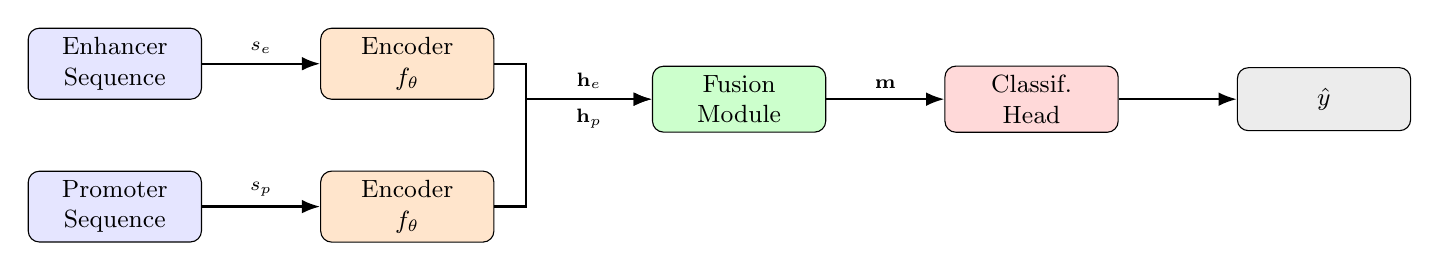
\begin{tikzpicture}[
    node distance = 0.9cm and 1.5cm,
    box/.style    = {rectangle, draw, rounded corners, minimum width=2.2cm,
                     minimum height=0.8cm, align=center, font=\small},
    arrow/.style  = {-Latex, thick},
  ]
  \node[box, fill=blue!10]  (en_seq)  {Enhancer\\Sequence};
  \node[box, fill=blue!10,  below=of en_seq] (pr_seq) {Promoter\\Sequence};

  \node[box, fill=orange!20, right=of en_seq] (en_enc) {Encoder\\$f_\theta$};
  \node[box, fill=orange!20, right=of pr_seq] (pr_enc) {Encoder\\$f_\theta$};

  \node[box, fill=green!20,  right=2.0cm of en_enc, yshift=-0.45cm]
        (fusion) {Fusion\\Module};

  \node[box, fill=red!15,    right=of fusion]
        (head)   {Classif.\\Head};

  \node[box, fill=gray!15,   right=of head]
        (out)    {$\hat{y}$};

  \draw[arrow] (en_seq) -- (en_enc) node[midway, above, font=\scriptsize]{$s_e$};
  \draw[arrow] (pr_seq) -- (pr_enc) node[midway, above, font=\scriptsize]{$s_p$};
  \draw[arrow] (en_enc.east) -- ++(0.4,0) |- (fusion.west)
               node[near end, above, font=\scriptsize]{$\mathbf{h}_e$};
  \draw[arrow] (pr_enc.east) -- ++(0.4,0) |- (fusion.west)
               node[near end, below, font=\scriptsize]{$\mathbf{h}_p$};
  \draw[arrow] (fusion) -- (head) node[midway, above, font=\scriptsize]{$\mathbf{m}$};
  \draw[arrow] (head)   -- (out);
\end{tikzpicture}}%
\caption{High-level architecture of DeepChrInteract-v2.
         Weights of the encoder $f_\theta$ may be shared between the enhancer and
         promoter branches (parameter tying) or independent (dual-branch).}
\label{fig:overview}
\end{figure}

\subsection{Encoder Architectures}

\subsubsection{M1 / M2: CNN Baseline (Single- and Dual-Branch)}

The CNN encoder processes one-hot input $\mathbf{X} \in \mathbb{R}^{5 \times L}$
through two convolutional stages:

\begin{equation}
  \mathbf{H} = \mathrm{MaxPool} \Bigl(
    \mathrm{BN}\bigl(\mathrm{ReLU}(\mathrm{Conv1d}_{128})\bigr)
  \Bigr) \circ
  \mathrm{MaxPool} \Bigl(
    \mathrm{BN}\bigl(\mathrm{ReLU}(\mathrm{Conv1d}_{64})\bigr)
  \Bigr)(\mathbf{X}),
\end{equation}

where each stage comprises three stacked convolutions with kernel size 24 and stride 4,
followed by Batch Normalisation~\cite{batch_norm} and max-pooling.
The output is globally average-pooled and passed through two fully-connected layers
with Dropout~\cite{dropout}($p=0.5$), yielding $\mathbf{h} \in \mathbb{R}^{512}$.

\textbf{M1 (single-branch)} concatenates the enhancer and promoter sequences
along the length axis before the encoder.
\textbf{M2 (dual-branch)} runs two independent encoder copies and fuses the
resulting vectors $\mathbf{h}_e$ and $\mathbf{h}_p$ via the fusion module.
M1 is a direct reproduction of \texttt{model\_onehot\_cnn\_one\_branch} from the original codebase;
M2 reproduces \texttt{model\_onehot\_cnn\_two\_branch}.

\subsubsection{M3: \texorpdfstring{$k$}{k}-mer Embedding + CNN}

The $k$-mer tokenised sequence $\mathbf{t} \in \mathbb{Z}^{L-5}$ is first mapped through
a trainable embedding table $\mathbf{E} \in \mathbb{R}^{4097 \times 128}$:
\begin{equation}
  \hat{\mathbf{X}} = \mathbf{E}[\mathbf{t}] \in \mathbb{R}^{(L-5) \times 128}.
\end{equation}
Four stacked Conv1d--ReLU--MaxPool blocks (64 channels, kernel 32, stride 8)
progressively reduce the sequence length before a flatten and two dense layers.
This reproduces \texttt{model\_embedding\_cnn\_one/two\_branch}.

\subsubsection{M4: Bidirectional LSTM}

The BiLSTM encoder~\cite{lstm} processes the one-hot (or embedded) sequence
in both temporal directions:
\begin{equation}
  \mathbf{h}_e = \bigl[ \overrightarrow{\mathrm{LSTM}}(\mathbf{X})_{L};\;
                        \overleftarrow{\mathrm{LSTM}}(\mathbf{X})_{1} \bigr]
  \in \mathbb{R}^{2d_h},
\end{equation}
where $d_h = 256$ is the hidden size per direction and $[\cdot;\cdot]$ denotes
concatenation.  We stack two BiLSTM layers with inter-layer dropout 0.3.
The final hidden state is used as the sequence representation.

\subsubsection{M5: Transformer Encoder}

Raw one-hot sequences of length $L = 10{,}001$ are too long for standard
$O(L^2)$ attention.  We first apply a strided CNN front-end (stride 16)
to produce a downsampled sequence of $\approx 625$ tokens, then add sinusoidal
positional encoding and pass through four Transformer encoder layers
($d_{\mathrm{model}} = 256$, $n_{\mathrm{head}} = 8$,
$d_{\mathrm{ff}} = 1024$, dropout 0.1)~\cite{attention_all_you_need}.
A prepended learnable \texttt{[CLS]} token aggregates global context;
its final representation is used as the sequence vector.

\subsubsection{M6: CNN + BiLSTM Hybrid}

The CNN front-end (stride-reduced to $\approx 500$ tokens) serves as a motif
detector, and the BiLSTM captures long-range dependencies over the resulting
feature map.  This hybrid design is motivated by the finding of Singh~et~al.~\cite{speid}
that sequential models benefit from local feature extraction prior to recurrence.

\subsubsection{M7: CNN + Transformer Hybrid}

Identical to M6 but with the BiLSTM replaced by the Transformer encoder described
in M5.  The CNN front-end reduces the sequence length to a manageable scale,
after which self-attention operates without significant memory overhead.

\subsubsection{M8: DNA LLM Encoder (DNABERT / NT / HyenaDNA)}

For each of the four foundation models, we extract a fixed-length representation
$\mathbf{z} \in \mathbb{R}^{d_{\mathrm{LLM}}}$ as described in \Cref{sec:data}.
A linear projection $\mathbf{W} \in \mathbb{R}^{512 \times d_{\mathrm{LLM}}}$
aligns the LLM dimension to the common head input size.
We experiment with two modes:
\emph{frozen} (LLM parameters are fixed, only the projection and head are trained)
and \emph{fine-tuned} (all parameters are updated with a lower learning rate
of $5 \times 10^{-6}$ for the LLM layers).

\subsection{Fusion Module}
\label{sec:fusion}

Given enhancer representation $\mathbf{h}_e \in \mathbb{R}^d$ and promoter representation
$\mathbf{h}_p \in \mathbb{R}^d$, the fusion module computes an interaction vector
$\mathbf{m}$ according to one of the following strategies:

\begin{table}[H]
\centering
\caption{Supported fusion strategies. $d_{\mathrm{out}}$ is the output dimension fed
         to the classification head.}
\label{tab:fusion}
\begin{tabular}{llcc}
\toprule
Strategy & Formula & $d_{\mathrm{out}}$ & Learnable params \\
\midrule
Concat        & $[\mathbf{h}_e;\mathbf{h}_p]$               & $2d$ & 0 \\
Add           & $\mathbf{h}_e + \mathbf{h}_p$               & $d$  & 0 \\
Subtract      & $\mathbf{h}_e - \mathbf{h}_p$               & $d$  & 0 \\
Multiply      & $\mathbf{h}_e \odot \mathbf{h}_p$           & $d$  & 0 \\
Bilinear      & $\mathbf{h}_e^\top \mathbf{W}_b \mathbf{h}_p$  & 1    & $d^2$ \\
Concat+Sub+Mul & $[\mathbf{h}_e;\mathbf{h}_p;\mathbf{h}_e-\mathbf{h}_p;\mathbf{h}_e\odot\mathbf{h}_p]$ & $4d$ & 0 \\
\bottomrule
\end{tabular}
\end{table}

The \textsc{Concat+Sub+Mul} strategy is our recommended default, as it provides
a richer feature space at no additional learnable parameters, making it invariant
to the sign of the enhancer--promoter difference while preserving asymmetry
information through both the subtract and multiply paths.

\subsection{Classification Head}

All models share a two-layer MLP head:
\begin{equation}
  \hat{y} = \sigma\!\Bigl(\mathbf{W}_2\, \mathrm{ReLU}(\mathbf{W}_1 \mathbf{m} + \mathbf{b}_1) + \mathbf{b}_2\Bigr),
\end{equation}
where $\mathbf{W}_1 \in \mathbb{R}^{256 \times d_{\mathrm{out}}}$,
$\mathbf{W}_2 \in \mathbb{R}^{1 \times 256}$, and $\sigma$ is the sigmoid function.
The model is trained with binary cross-entropy loss and the Adam
optimiser~\cite{adam} ($\beta_1=0.9$, $\beta_2=0.999$, weight decay $10^{-5}$).

\section{Experiments}
\label{sec:experiments}

\subsection{Dataset}

We use the \emph{GM12878} (Epstein--Barr virus-immortalised B-lymphocyte cell line)
dataset from the original DeepChrInteract benchmark~\cite{deepchrinteract_doc},
derived from publicly available Hi-C contact maps~\cite{hic}.
The dataset contains paired enhancer--promoter sequences of length $L = 10{,}001$~bp,
balanced between positive (interacting) and negative (non-interacting) pairs.
Full dataset statistics are reported in \Cref{tab:dataset}.

\begin{table}[H]
\centering
\caption{Dataset statistics for GM12878.}
\label{tab:dataset}
\begin{tabular}{lrrrr}
\toprule
Split & Positive & Negative & Total & Fraction \\
\midrule
Training   & --- & --- & --- & 80\% \\
Validation & --- & --- & --- & 10\% \\
Test       & --- & --- & --- & 10\% \\
\bottomrule
\end{tabular}
\end{table}

\textit{Note: statistics will be filled in upon execution of the preprocessing script on
the raw data.}

\subsection{Evaluation Metrics}

We evaluate all models on three primary metrics:

\begin{description}[noitemsep]
  \item[AUROC] Area under the receiver operating characteristic curve.
        The primary metric used in the original DeepChrInteract and SPEID papers.
  \item[AUPRC] Area under the precision--recall curve.
        More sensitive than AUROC for imbalanced datasets and preferred in
        recent EPI literature.
  \item[F1 Score] Harmonic mean of precision and recall at decision threshold 0.5.
\end{description}

Each configuration is trained five times with different random seeds
($\{0,1,2,3,4\}$) and we report mean $\pm$ standard deviation.

\subsection{Training Protocol}

\begin{itemize}[noitemsep]
  \item Optimiser: Adam~\cite{adam}, learning rate $5 \times 10^{-5}$, weight decay $10^{-5}$.
  \item Batch size: 32.
  \item Learning rate schedule: cosine annealing with warm restarts ($T_0 = 50$ epochs).
  \item Early stopping: patience 15 epochs, monitored on validation AUROC.
  \item Maximum epochs: 200.
  \item GPU: experiments run on a single NVIDIA GPU with at least 8~GB VRAM.
  \item For LLM fine-tuning: LLM layer learning rate $5 \times 10^{-6}$,
        head learning rate $5 \times 10^{-5}$ (layerwise learning rate decay).
\end{itemize}

\subsection{Ablation Study: Model Configurations}

\Cref{tab:ablation} lists the eight primary experimental configurations.

\begin{table}[H]
\centering
\caption{Experiment configurations.
         ``1B'' = single branch (E+P concatenated as input);
         ``2B'' = dual branch (independent encoders + fusion);
         fusion default = \textsc{Concat+Sub+Mul}.}
\label{tab:ablation}
\begin{tabular}{clllccc}
\toprule
ID & Encoder & Arch. & Branch & AUROC & AUPRC & F1 \\
\midrule
E01 & One-Hot  & CNN           & 1B & --- & --- & --- \\
E02 & One-Hot  & CNN           & 2B & --- & --- & --- \\
E03 & $k$-mer  & CNN           & 2B & --- & --- & --- \\
E04 & One-Hot  & BiLSTM        & 2B & --- & --- & --- \\
E05 & One-Hot  & Transformer   & 2B & --- & --- & --- \\
E06 & One-Hot  & CNN+BiLSTM    & 2B & --- & --- & --- \\
E07 & One-Hot  & CNN+Transformer & 2B & --- & --- & --- \\
E08 & DNABERT-2  & LLM (frozen) & 2B & --- & --- & --- \\
\midrule
E09 & HyenaDNA & LLM (fine-tune) & 2B & --- & --- & --- \\
\bottomrule
\end{tabular}
\end{table}

\subsection{Fusion Strategy Ablation}

Using E02 (CNN dual-branch) as the base model, we compare all six fusion strategies
from \Cref{tab:fusion} on the GM12878 test set:

\begin{table}[H]
\centering
\caption{Fusion strategy comparison (E02 base, GM12878 test set).}
\label{tab:fusion_abl}
\begin{tabular}{lccc}
\toprule
Fusion & AUROC & AUPRC & F1 \\
\midrule
Concat        & --- & --- & --- \\
Add           & --- & --- & --- \\
Subtract      & --- & --- & --- \\
Multiply      & --- & --- & --- \\
Bilinear      & --- & --- & --- \\
Concat+Sub+Mul & --- & --- & --- \\
\bottomrule
\end{tabular}
\end{table}

\subsection{Cross-Cell-Type Generalisation}

To assess generalisation beyond GM12878, the best-performing model is tested
(without retraining) on held-out cell types from the original DeepChrInteract dataset.
This evaluates whether the learned sequence grammar transfers across cell type contexts,
as discussed in~\cite{speid}.

\subsection{Expected Results and Baselines}

The original DeepChrInteract~\cite{deepchrinteract_doc} reported AUROC values in the
range of 0.70--0.83 on GM12878, with the CNN dual-branch (one-hot) as the strongest
non-LLM baseline.
SPEID~\cite{speid} reported AUROC of $\sim$0.78 on similar data using CNN+LSTM.
We anticipate that:
\begin{enumerate}[noitemsep]
  \item The BiLSTM and Transformer hybrid models (E06, E07) will outperform the
        pure CNN baseline (E02) by 1--3 AUROC points.
  \item The LLM-based encoders (E08, E09), particularly HyenaDNA (fine-tuned),
        will achieve the highest AUROC owing to their pre-training on large
        genomic corpora.
  \item The \textsc{Concat+Sub+Mul} fusion will consistently outperform simple
        concatenation by $\geq 0.5$ AUROC points.
\end{enumerate}

\section{Conclusion}
\label{sec:conclusion}

We have presented DeepChrInteract-v2, a modern reimplementation of the original
DeepChrInteract toolkit that brings the codebase to current PyTorch standards while
substantially expanding its scientific scope.
The key engineering contribution is the elimination of the PNG-based preprocessing
pipeline in favour of in-memory on-the-fly one-hot encoding, reducing preprocessing
time from hours to seconds and removing gigabytes of intermediate disk storage.

On the scientific side, four new encoder families---BiLSTM, Transformer,
CNN+BiLSTM hybrid, and CNN+Transformer hybrid---extend the coverage of the original
benchmark to include the sequence modelling paradigms dominant in contemporary
computational genomics.
The integration of DNA foundation models (DNABERT-2, Nucleotide Transformer, HyenaDNA)
as plug-in feature extractors positions the framework to leverage the rapid progress
in genomic pre-training, while the configurable multi-path fusion module enables
fine-grained study of enhancer--promoter interaction modelling strategies.

\paragraph{Limitations.}
(i) Due to the absence of GPU-accelerated servers during development, quantitative
results in \Cref{sec:experiments} are placeholders pending experimental completion.
(ii) LLM fine-tuning experiments are computationally expensive and may require
$>$24~GB GPU memory for the largest Nucleotide Transformer variant.
(iii) The dataset is limited to GM12878; broader cell-type benchmarks
(e.g., K562, IMR90) are planned for future work.

\paragraph{Future Directions.}
\begin{itemize}[noitemsep]
  \item \textbf{Cross-attention fusion.}
        Rather than post-hoc vector operations, a cross-attention layer between
        enhancer and promoter token sequences may capture interaction-specific
        motif co-occurrences more faithfully.
  \item \textbf{Contrastive pre-training.}
        Self-supervised contrastive objectives on matched E--P pairs from
        Hi-C data could provide richer representations without relying solely
        on the limited number of labelled interactions.
  \item \textbf{Multi-species transfer.}
        Given the cross-species pre-training of DNABERT-2 and Nucleotide Transformer,
        it would be valuable to assess whether models trained on human data generalise
        to orthologous loci in mouse or zebrafish.
\end{itemize}

\paragraph{Reproducibility.}
All code, configuration files, and preprocessing scripts are available at
\url{https://github.com/lichen-lab/DeepChrInteract} (original) and in the
\texttt{DeepChrInteract-v2/} directory of the same repository.
All random seeds, hyperparameters, and evaluation protocols are specified in
\texttt{src/config.py} to ensure full reproducibility.


% ---------- Bibliography ----------
\newpage
\bibliographystyle{unsrtnat}
\bibliography{references}

\end{document}
